\chapter{Methoden}
\label{chapter:methods}

\section{Human Centered Design}
Human Centered Design ist eine Methode die den Entwicklungsprozess von
interaktiven Systemen und Software beschreibt. Die Kernthese ist hierbei, dass
die Nutzenden der Systeme und ihr Umfeld im Mittelpunkt aller Entwicklungs- und
Designprozesse stehen. Thematisch lässt sich die Theorie des Human Centered
Design in das Themenfeld der Mensch-Maschine Interaktion
einordnen.\cite{HMI-HCD}

Die Entwicklung von Software war in den Anfängen geprägt von den technisch sehr
eingeschränkte Möglichkeiten des Computers. Software wurde also größtenteils so
entwickelt, dass sie möglichst problemlos und effizient auf dem entsprechenden
Computer ausgeführt werden kann. Alle Entwicklungsprozesse wurden also aus
Perspektive der ausführenden Maschine gedacht. Der Ansatz des Human Centered
Design setzt dieser maschinenzentrierten Vorgehensweise eine klare Alternative
entgegen. Martin Ludwig Hofmann beschreibt den Grundgedanken in \textit{Human
    Centered Design} so: \glqq{} [Es geht] nicht darum, mit Geräten zu denken,
sondern mit Menschen und ihren Weltanschauungen\grqq{}\cite{hcd}. Wie in
Kapitel \ref{chapter:introduction} erläutert, gewinnt dieser Ansatz in der
heutigen Zeit immer größere Bedeutung. Wie Alan Dix in \textit{Human Computer
    Interaction} erklärt, hat sich die Art und Weise, wie Menschen und Computer
interagieren, in den letzten Jahrzehnten stark verändert. Während Computer
früher meist nur mathematische Berechnungen durchführten, sind Softwaresysteme
heute hochgradig interaktiv und sollen von allen Teilen der Gesellschaft
ungehindert genutzt werden können\cite{hci}.

Um die Methodik des Human Centered Design weiter zu spezifizieren ist zunächst
festzuhalten, dass dem Designprozess an sich eine wichtige Rolle zugeschrieben
wird. Es reicht nicht aus, dass eine Software korrekt funktioniert, sich also
alle Berechnungen und Prozesse fehlerfrei ausführen lassen. Im Human Centered
Design liegt der Fokus auf der Interaktion zwischen dem Menschen und der
Maschine. In Abgrenzung zum \textit{User Centered Design} werden beim Human
Centered Design nicht nur die unmittelbaren Nutzenden mit einbezogen. Alle
Personen, die von der Gestaltung der Systeme betroffen sind sollen während des
Designprozesses beachtet werden.\cite{sequenceDiagrams} Man betrachtet, wie die
Menschen mit dem Computer interagieren. Wie stoßen sie Prozesse an? Welche
Reaktionen erwarten sie von dem System? Die Betroffenen sollen mit den Systemen
möglichst intuitiv interagieren können. Die Benutzeroberfläche der Software
soll selbst erklären, welche Funktionen auf welchem Weg erreicht werden können.
Ein essentieller Bestandteil hierfür ist zu verstehen, wie die Systeme genutzt
werden. Relevante Fragestellung sind hier: In welchem Kontext werden die
Systeme eingesetzt? Welche Menschen arbeiten mit den Systemen? Welche
Informationen müssen die Nutzenden schnell erfassen können? Um diese Fragen
sinnvoll beantworten zu können müssen die Betroffenen während der Designphase
kontinuierlich in den Entwicklungsprozess einbezogen werden. Ihre gesamte
Situation, sowie ihre Bedürfnisse müssen im Designprozess untersucht und direkt
in das Produktdesign integriert werden.\cite{hci}

Wie M. Kurosu erwähnt, ist ein weiterer wichtiger Aspekt des Human Centered
Design das Durchlaufen mehrere Iterationen. Ein Produkt ist nach einem ersten
Entwicklungszyklus selten schon perfekt. Oftmals ist es wichtig den Betroffenen
erste Ergebnisse zu präsentieren oder ihnen Prototypen zu zeigen. Das Feedback,
das Nutzende hierbei geben, muss dokumentiert und für weitere Iterationen der
Entwicklung aufgearbeitet werden. Wie Kurosu weiter erwähnt, steht der
zyklische Ablauf des Human Centered Design auch in der entsprechende ISO Norm
im Fokus.\cite{kurosuHCI}

\begin{figure}[H]
    \caption{Iteratives Vorgehen im Human Centered Design nach ISO 9241 \cite{iso9241}}
    \centering
    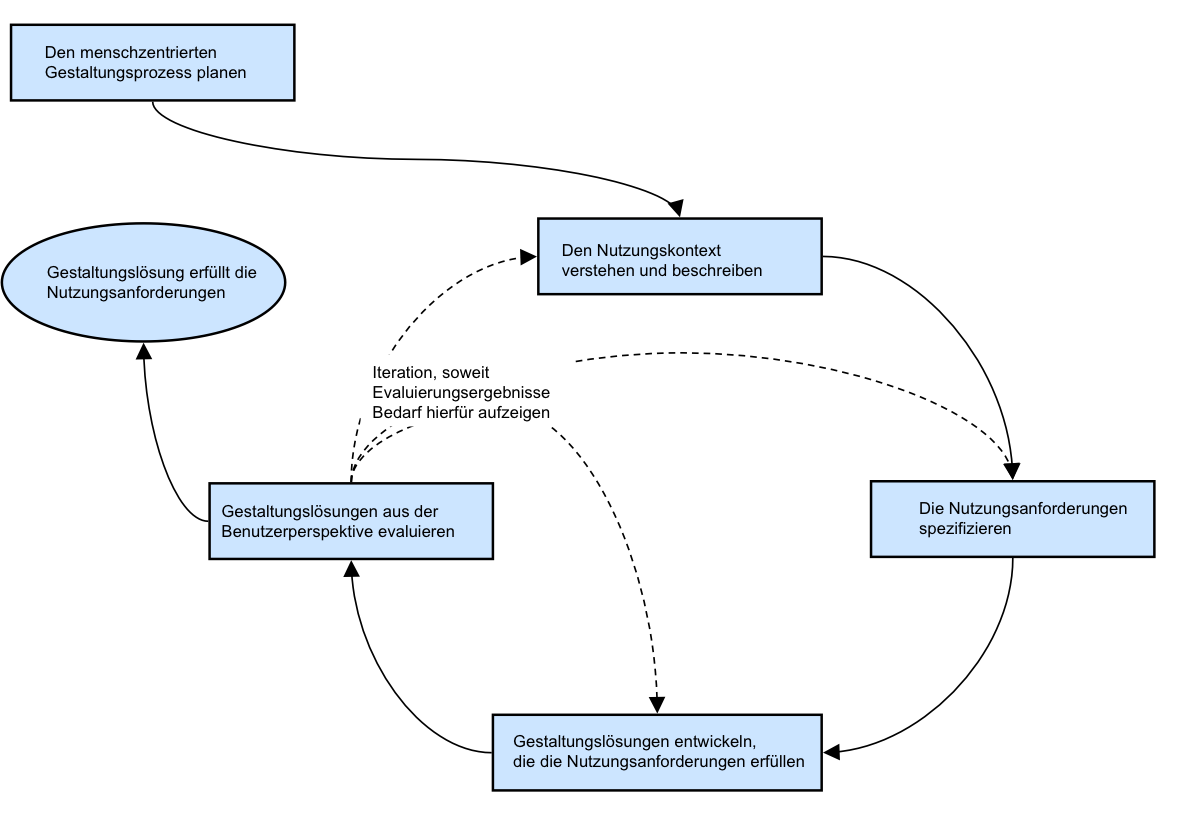
\includegraphics[width=10cm]{HCD.png}
\end{figure}

Das Schaubild der Iso Norm verdeutlicht den Ablauf eines Designprozesses in
mehreren Phasen. Nachdem geplant ist, was für ein Projekt umgesetzt werden soll
beginnt der zyklische Kreislauf des Entwicklungsprozesses. Im ersten Schritt
liegt der Fokus auf dem Analysieren der Situation, in der das zu entwickelnde
System später eingesetzt werden soll. Nur wer den Kontext eines interaktiven
Systems kennt, kann die Schnittstelle zwischen Maschine und Mensch adäquat
gestalten. Im zweiten Schritt geht es darum aus den geplanten Erwartungen an
das System und der Analyse des Nutzungskontextes konkrete Anforderungen zu
formulieren. Hierbei steht noch nicht im Fokus, wie diese Anforderungen
technisch umgesetzt werden könnten. Vielmehr geht es darum, welche
Anforderungen das fertige System überhaupt erfüllen soll. Im dritten Schritt
geht es nun darum diese Anforderungen tatsächlich umzusetzen und technische
Lösungen zu implementieren. Gibt es erste Ergebnisse wird der vierte Schritt
relevant: Die umgesetzten Lösungen müssen im tatsächlichen Nutzungskontext
evaluiert werden. Das setzt wieder eine intensiven Austausch mit den
Betroffenen des Systems voraus. Mit dem so gewonnen Feedback kann der Prozess
wieder von vorne beginnen. Fehlende Features können nachgebessert,
missverständliche Schnittstellen klarer gestaltet und Probleme im praktischen
Einsatz minimiert werden.\cite{iso9241}

G.A. Boy berichtet in \textit{The Handbook of Human-Machine Interaction} wie
wichtig es ist, dem späteren Nutzenden der System erste Prototypen und Ideen zu
präsentieren. Oftmals wissen die Nutzenden gar nicht welche technischen
Möglichkeiten es gibt oder welche alternativen Bedienkonzepte in ihrem Kontext
besonders gut funktionieren könnten. Im Mittelpunkt steht also das Zuhören und Eingehen auf die
Nutzenden und ihr Umfeld. Allerdings kann auch das Einbringen neuer, für die Nutzenden
unbekannter Lösungsansätze, von hoher Bedeutung sein.\cite{HMI-HCD}

\section{Interview im Kontext}

Ein wesentlicher Bestandteil im Entwicklungsprozess nach den Methoden des Human
Centered Design ist der intensive Austausch mit den Betroffenen der Systeme.
Hierfür ist es wichtig, dass Softwareentwickler und Designer von
Benutzerschnittstellen in den direkten Austausch mit den Nutzenden der Systeme
gehen. Um diesen Prozess strukturiert und zielführend zu durchlaufen, kann
hierfür die Methode des \textit{Interviews im Kontext} benutzt werden.

Beim Interview im Kontext geht es darum, die Nutzenden der Systeme in dem
Umfeld zu beobachten, in dem die Software tatsächlich auch im praktischen
Alltag eingesetzt wird. Der Fokus liegt also auf dem Umfeld der Interaktion mit
technischen Systemen. In herkömmliche Interviews begegnen sich Interviewer und
Interviewter oftmals in einer neutralen Umgebung, wie beispielsweise einem
Konferenzraum und sprechen über die Prozesse für die sich der Interviewende
interessiert. Beim Interview im Kontext geht es nicht darum \textbf{über} einen
Prozess zu sprechen, sondern den Prozess als Interviewender \textbf{direkt
    mitzuerleben}\cite{contextualDesign}. In \textit{Manual on Human-Computer
    Interaction} legen die Autoren den Fokus auf die genaue Beobachtung der
NuTzenden in der Interaktion mit den Systemen. Mit dieser Methode könne man
noch viel mehr praxisnahe Details erfassen, als wenn man mit den Nutzenden nur
über das System spricht. Spricht man mit Nutzenden beispielsweise darüber wie
sie eine Software bedienen, gibt es möglicherweise viele Dinge, die sie nicht
erwähnen, weil sie vergessen wurden, nicht relevant erscheinen oder Nutzende
nicht wissen, wie sie genau darüber sprechen sollen\cite{hciHandbook}.

Dies kann in der Praxis bedeuten, dass man sich mit den Nutzenden der Systeme
in ihren Büroräumen trifft und für mehrere Stunden mit dabei ist, wenn sie
ihrer Arbeit nachgehen und mit den technischen Systemen interagieren. Die Rolle
des Interviewenden ist dabei aus einer beobachtenden Perspektive zu verstehen.
Der Interviewte soll die Richtung bestimmen, in die sich das Interview
entwickelt. Der Interviewende hört hauptsächlich zu und beobachtet wie die
Personen in ihrer Umgebung, ihrem Kontext agieren\cite{hciHandbook}. Dazu kann
der Interviewende Notizen machen um eine spätere Auswertung des Interviews zu
erleichtern. An passenden Stellen kann der Interviewende gezielte Nachfragen
stellen um beispielsweise Hürden bei der Interaktion mit den Systemen zu
provozieren. Eine weitere Intention für Nachfragen kann aber auch sein, die
Gedanken und Emotionen des Nutzenden zu erfragen, welche er beim Benutzen des
Systems empfindet.

\begin{figure}[h]
    \caption{Während eines Interviews im Kontext können viele Aspekte beobachtet werden, die über das benutzte System selbst hinausgehen\cite{johannesGrafik}}
    \centering
    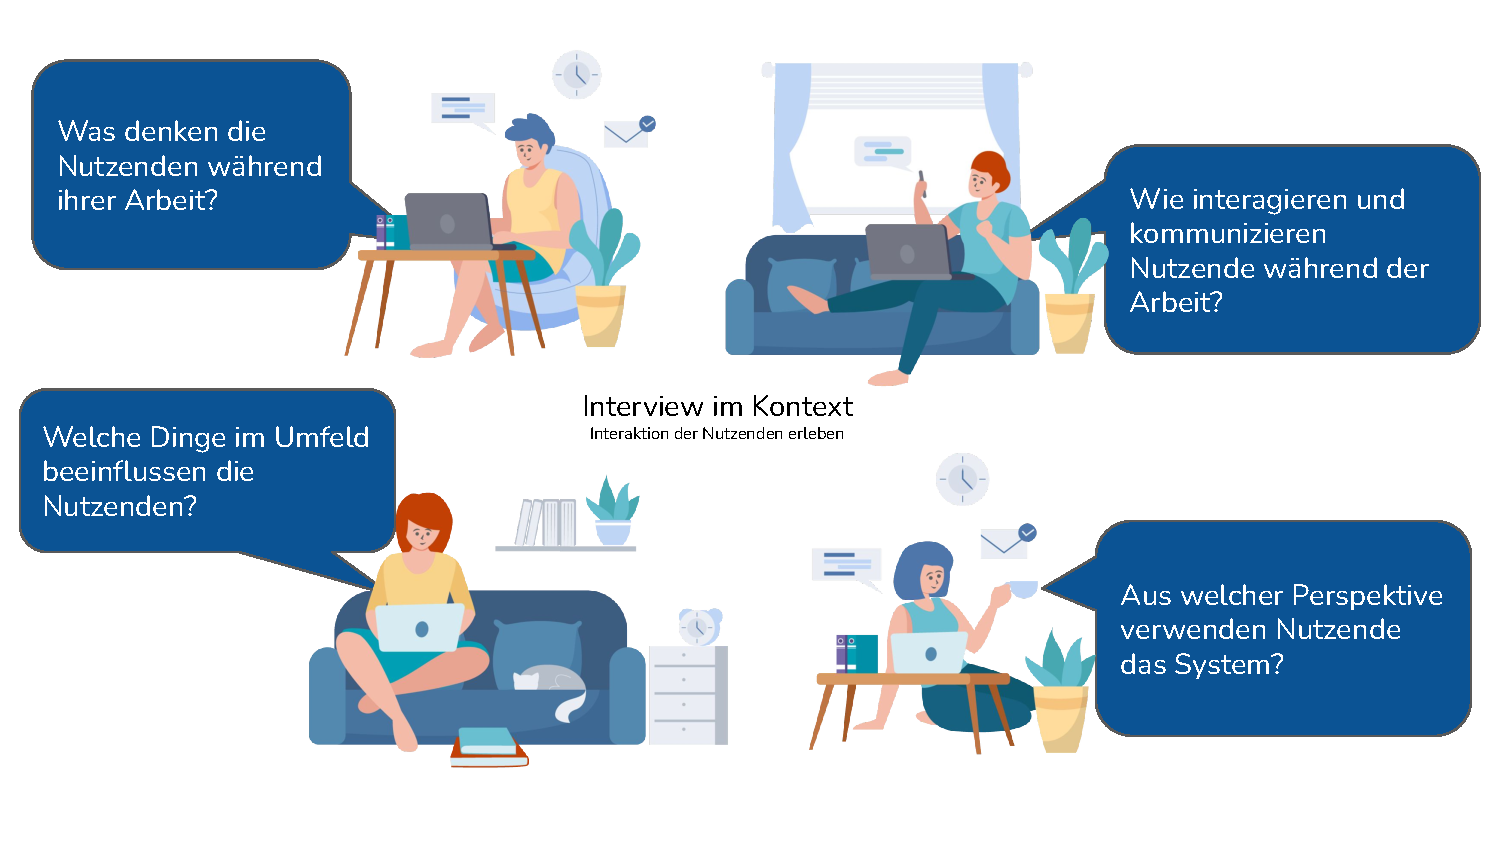
\includegraphics[width=0.9\textwidth]{Interview im Kontext Schaubild.pdf}
\end{figure}

Das Ergebnis eines Interviews im Kontext ist also eine ausführliche Beobachtung
der Interaktion von Nutzenden mit den entsprechenden Systemen im alltäglichen
Kontext. Diese Beobachtungen können schriftlich festgehalten werden oder auch
durch Video- und Tonaufzeichnungen ergänzt werden. Im Nachgang des Interviews
müssen die Beobachtungen ausgewertet und analysiert werden. Ziel ist es dabei
aus den Beobachtungen des Interviews konkrete Nutzungsanforderung an das zu
entwickelnde System zu formulieren\cite{HMI-HCD}. Hier können beispielsweise Featurelisten,
Sequenzdiagramme oder User-Scenarios zum Einsatz kommen\cite{sequenceDiagrams}.